\documentclass[ignorenonframetext]{beamer}
%\documentclass[11pt]{article}
%\usepackage{beamerarticle}
\mode<article>{\usepackage{fullpage}
  \usepackage{palatino}
  \usepackage{mathpazo}
  \usepackage{graphicx}
}

\mode<presentation>{\usetheme{Boadilla}}

\usepackage[latin1]{inputenc}
\usepackage{amsmath}

\title[Physics for National Security]{Physics for National Security}
\subtitle{Spectral Comparison Ratio Anomaly Mapping\\(SCRAM)}
\author{Alex Reinhart}
\institute{Applied Research Labs}
\date{April 8, 2013}

\begin{document}

\maketitle

\begin{frame}
\titlepage
\end{frame}

What do I mean, physics for national security? Well, I mean this:

\begin{frame}
  \begin{figure}
    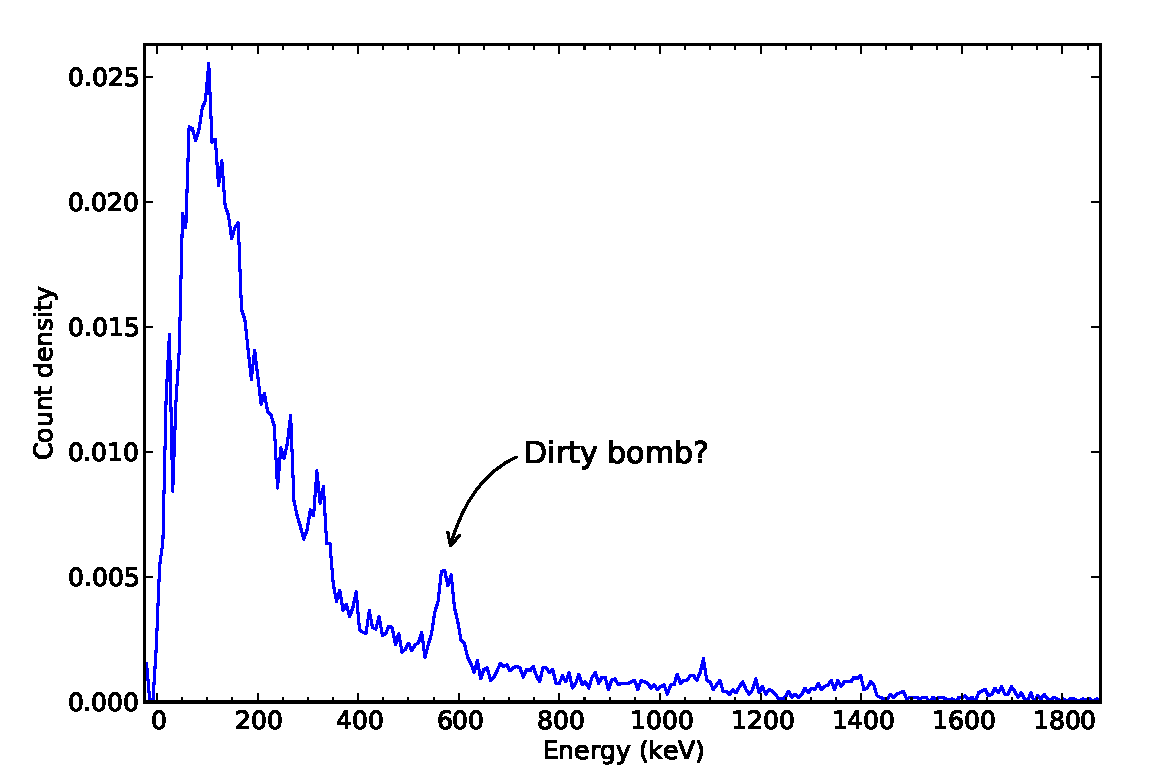
\includegraphics[width=110mm]{figures/talk-bomb-spectrum.pdf}
    \caption{Gamma ray spectrum collected at Pickle Research Campus.}
  \end{figure}
\end{frame}

That's a gamma ray spectrum I collected with a small scintillator detector at
PRC. Normally, you expect a big low-energy hump from Compton scattering and not
much else. But there's a peak, indicating that something nearby is undergoing
radioactive decay and shooting out gamma rays. What is it? How do we find the
source and tell if it's dangerous?

In this case, we knew the source: welds at a new chilling station were being
tested with gamma ray imaging, and the peak came from iridium-192 used in this
process. But there's not always a good excuse. We need a way to check on these
things.

\begin{frame}{Project goals}
  \begin{itemize}
    \item Inexpensive wide-area radiation surveillance
    \item Anomaly detection and mapping
    \item Isotope identification
  \end{itemize}
\end{frame}

We saw a need for a system that could map radiation over a wide area and detect
sudden changes. By ``surveillance'' I mean a system that can watch for days or
months, waiting for anything to change unexpectedly. Some police departments
already have radiation alert systems: UTPD officers wear pagers which alert them
when radiation levels suddenly increase, although the pager doesn't know if
that's normal or a bomb.

Unexpected changes can come from many sources. Many people undergo medical
treatments which use radioisotopes like iodine-131 and technetium-99m. UTPD has
stopped and questioned radioactive people before. Industrial radioactive sources
are sometimes used during construction or maintenance to inspect welds, and UTPD
has surrounded contractors with guns drawn when they forgot to file the right
paperwork before performing radiography. Some common sources:

\begin{frame}{Radiation sources}
  \begin{itemize}
    \item Natural stone (granite!) and brick
    \item Old red Fiestaware
    \item Bananas
    \item Medical cobalt-60 irradiators
    \item Fluorine-18, iodine-131, technetium-99m-dosed patients
    \item Industrial iridium-192 sources (sometimes stolen)
  \end{itemize}
  Industrial and medical sources are frequently poorly secured
\end{frame}

I say ``poorly secured.'' To quote a GAO report:

\begin{quote}
  At a hospital in a major U.S. city, we observed that the interior door to the
  hospital blood bank, which had a cesium-137 blood irradiator of approximately
  1,500 curies, had the combination to the lock written on the door frame. The
  door is in a busy hallway with heavy traffic...
\end{quote}

There's also a natural spatial variation in the background:

\begin{frame}
  \begin{figure}
    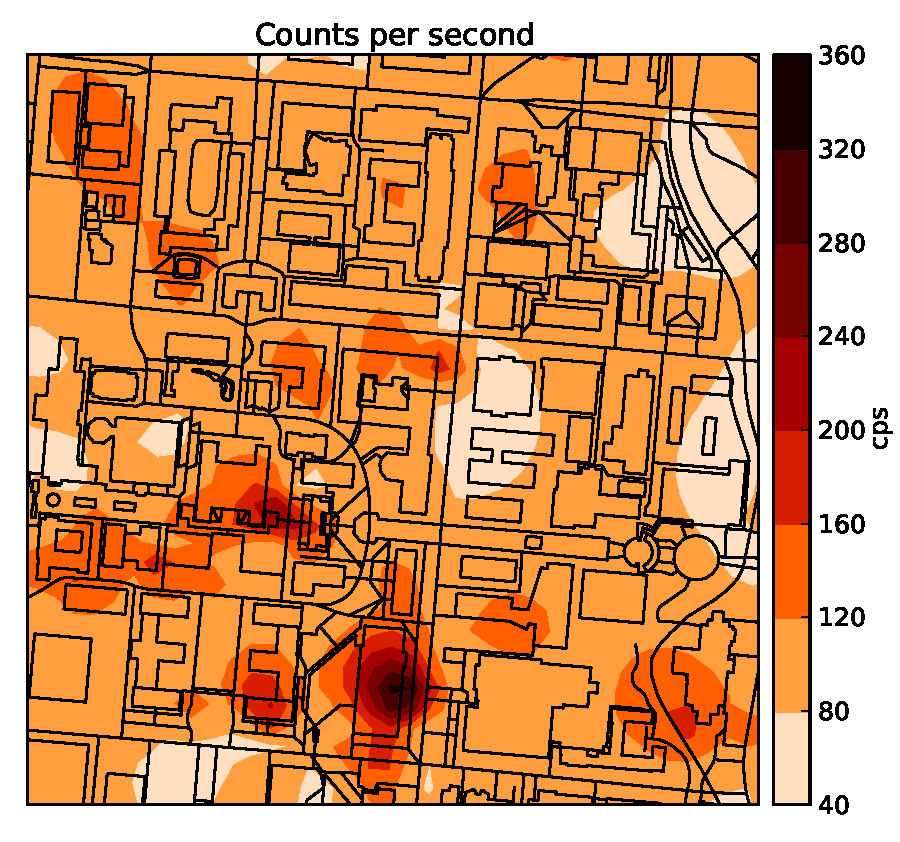
\includegraphics[width=85mm]{figures/talk-campus-map.pdf}
    \caption{The University of Texas campus radiation map.}
  \end{figure}
\end{frame}

Yeah, that's the business school.

If the background varies so much, it's hard to just put on a pager and detect
anomalies. There are too many natural anomalies. You want something that builds
a map like this one, then checks back the next day to see if it's changed. But
you don't want to just look at count rates, like this. You want to look at
spectra.

\begin{frame}
  \begin{figure}
    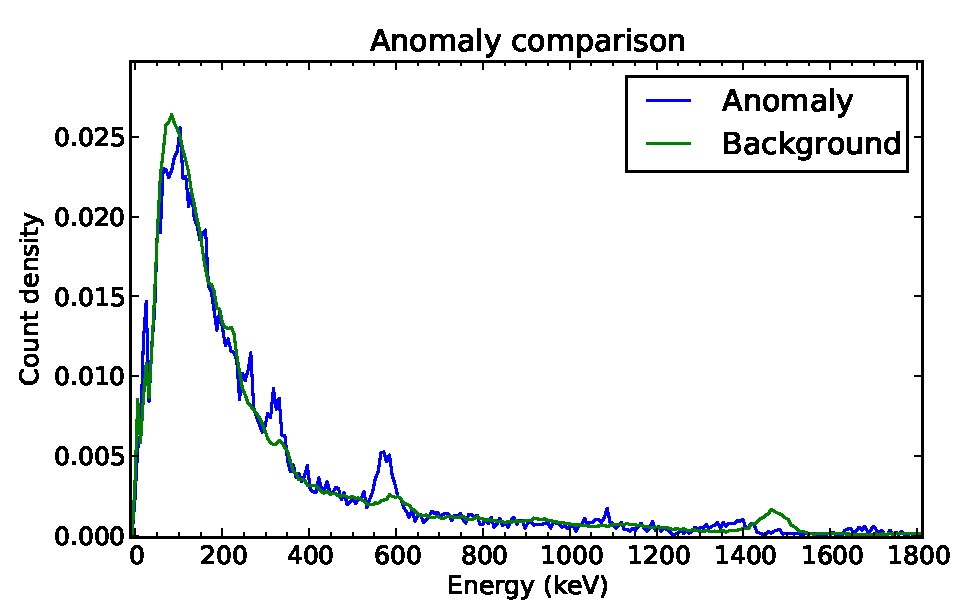
\includegraphics[width=120mm]{figures/talk-spectral-anomaly.pdf}
    \caption{``Normal'' and anomalous.}
  \end{figure}
\end{frame}

So how do we do it? Spectral comparison ratios. Divide the spectrum up into
bins. Maybe you choose the bins to cover regions of specific isotopes, or split
it equally, or whatever you'd like. Then:

\begin{frame}{Spectral comparison ratios}
  \begin{align*}
    \mathbf{c} &= \text{vector of counts}\\
    \mathbf{b} &= \text{background observation counts}\\
    s_i &= c_1 - \frac{b_1}{b_i} c_i\\
    D^2 &= \mathbf{s}^T \Sigma^{-1} \mathbf{s}
  \end{align*}
\end{frame}

\(D^2\) is our anomaly statistic. It should follow a \(\chi^2\)
distribution. But wait: what's \(\Sigma\)? It's the covariance matrix of
\(\mathbf{s}\) in all of our previous data. But covariance matrices require more
observations than variables to estimate accurately. That means if we have eight
energy bins we'd need to observe a region ten or twenty times before we can do
anomaly detection. That would suck.

\begin{frame}{Estimating \(\Sigma\)}
  \begin{itemize}
    \item Make an assumption: \(\text{var}(c_i) = V c_i\)
    \item In other words, assume gamma ray counts are (almost)
      Poisson-distributed
    \item Then, decompose:
      \begin{equation*}
        \Sigma_{ij} = \text{corr}(s_i, s_j) \sqrt{\text{var}(s_i)\, \text{var}(s_j)}
      \end{equation*}
    \item We can cheat and calculate \(\text{corr}(s_i, s_j)\) our data. What
      about \(\text{var}(s_i)\)?
  \end{itemize}
\end{frame}

I will spare you the details.

\begin{frame}{Estimating \(\Sigma\)}
  Use \(\text{var}(c_i) = V c_i\) and our equation for \(s_i\). Derive variance:
  \begin{equation*}
    \text{var}(s_i) = V \left(c_1 + \left(\frac{b_1}{b_i}\right)^2 c_i -
      2\frac{b_1}{b_i} \left(\frac{T_c}{T_b}\right)^2 \text{corr}(b_1, b_i)
      \sqrt{b_1 b_i}\right)
  \end{equation*}
  That was fun.
\end{frame}

Now, divide up space into blocks. Sum up all your observations in one block and
compare them to the observations you made yesterday in that block. 

\begin{frame}
  \begin{figure}
    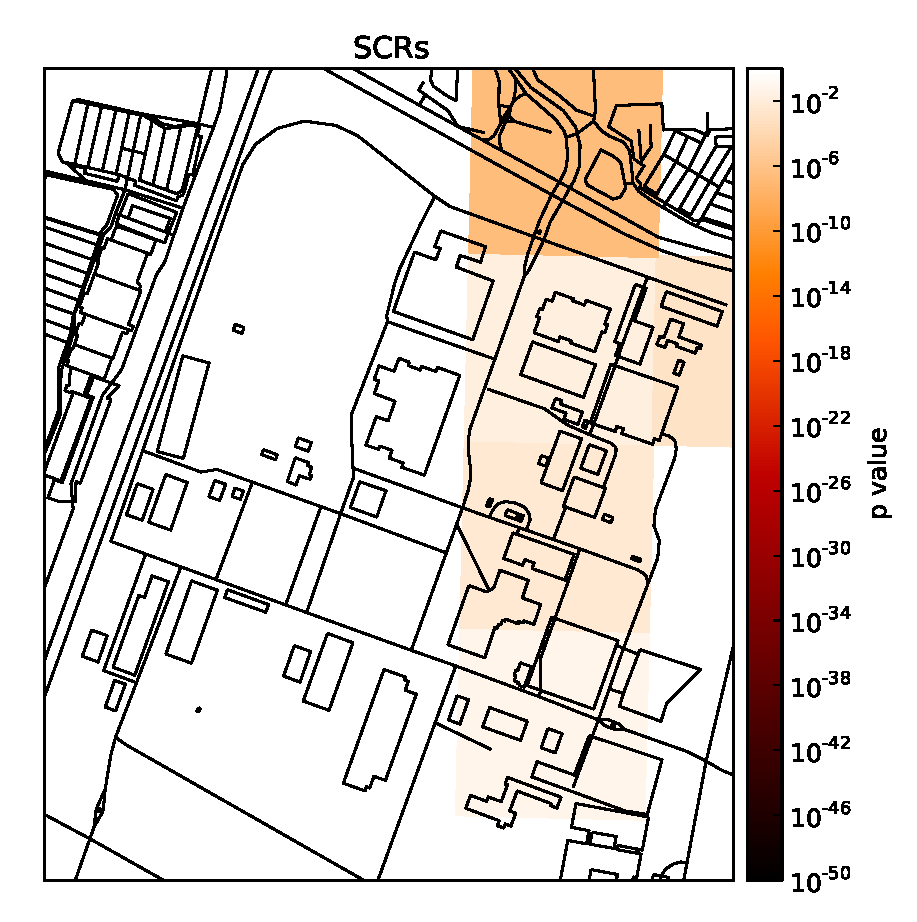
\includegraphics[width=90mm]{figures/talk-prc-preradiography-scr.pdf}
    \caption{Normal.}
  \end{figure}
\end{frame}

\begin{frame}
  \begin{figure}
    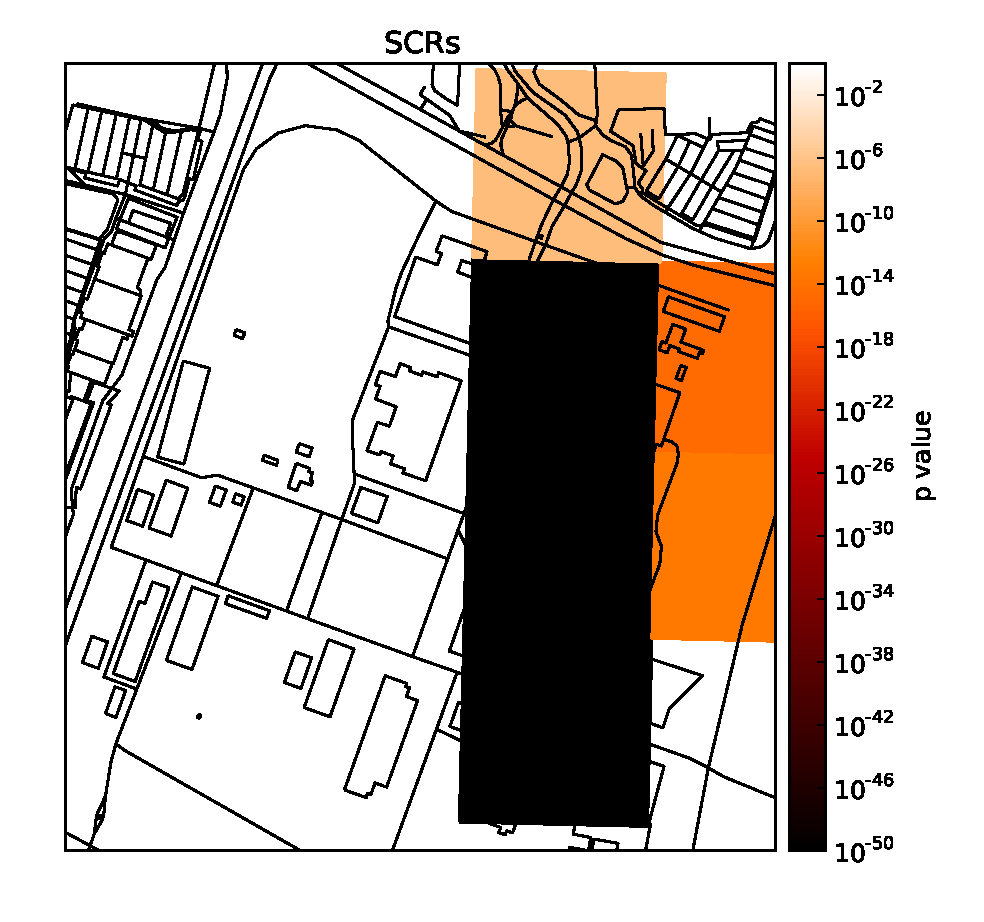
\includegraphics[width=93mm]{figures/talk-prc-radiography-scr.pdf}
    \caption{Abnormal.}
  \end{figure}
\end{frame}

How do I choose what size block to use?

\begin{frame}
  \begin{figure}
    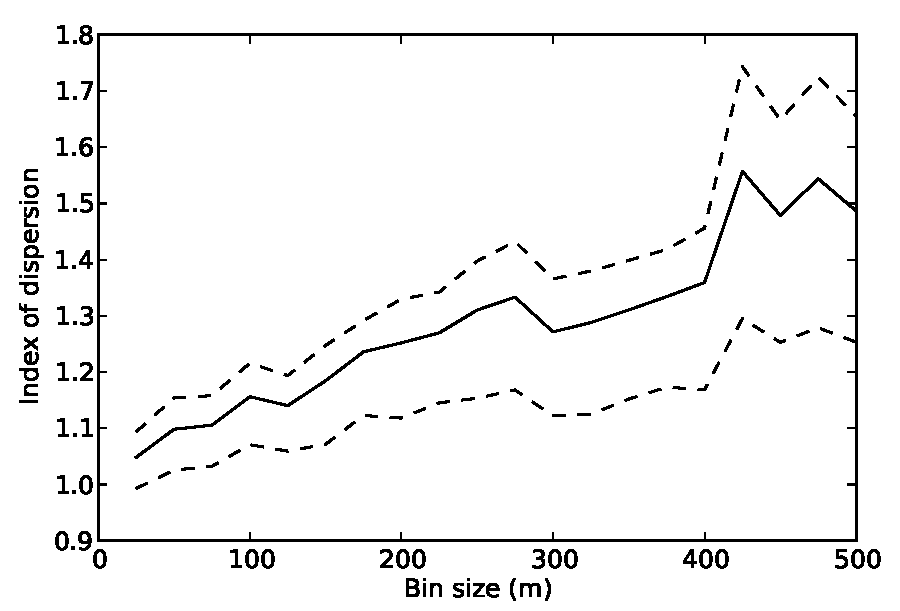
\includegraphics[width=100mm]{figures/poisson-dispersion.pdf}
    \caption{What I meant when I said ``almost'' Poisson-distributed.}
  \end{figure}
\end{frame}

The next thing we did was blind testing. We needed a place with radioactive
sources we could detect but didn't know about in advance. Now, we know there are
radioactive people -- with medical treatments and whatnot. So we need a place
where there are lots of people in one place, so the odds will be in favor of one
being radioactive.

Like a football game.

\begin{frame}
  \begin{figure}
    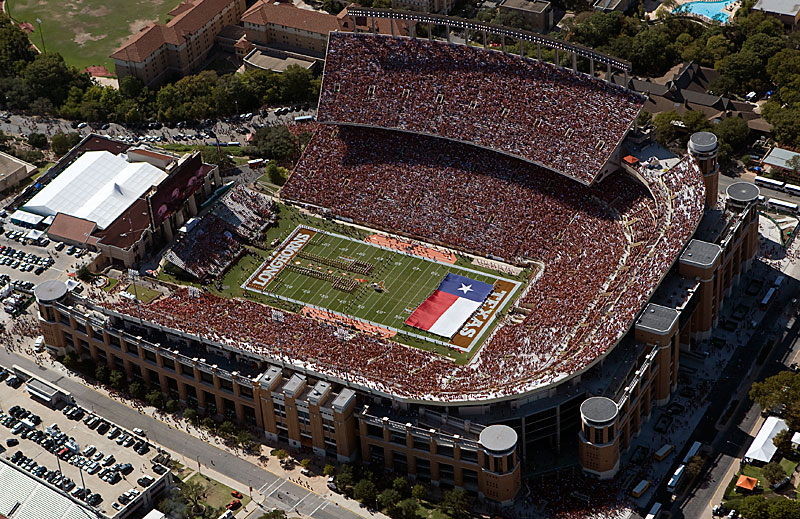
\includegraphics[width=100mm]{figures/talk-stadium.jpg}
    \caption{The Radiation Mapping Proving Grounds.}
  \end{figure}
\end{frame}

\begin{frame}{Stadium data collection}
  Imagine a map here.
\end{frame}

\end{document}